We consider the stationary Gaussian RF $\{r(\vect{x}) \ssep \vect{x} \in \mathrm{D} \subset \R^2\}$ with $\mathrm{D} \colon [(1,30), (1,30)]$,
%
\begin{align*}
    \E\{r(\vect{x})\} &= \mu_r = 0 \\
    \Var\{r(\vect{x})\} &= \sigma_r^2 \\
    \Corr\{r(\vect{x}), r(\vect{x'})\} &= \exp\{-\tau/\xi_r\}
\end{align*}
%
and $\tau = |\vect{x} - \vect{x'}|$.

%%%%%%%%%%%%%%%%%%%%%%%%%%%%%%%%%%%%%%%%%%%%%%%%%%%%%%%%%%%%%%%%%%%%%%
\paragraph{a)}
We consider the discretized Gaussian RF $\{r(\vect{x}) \ssep \vect{x} \in \mathrm{L}\}$ on the grid $\mathrm{L} \colon [30 \times 30] \in \mathrm{D}$ with model parameters $\sigma_r^2=2$ and $\xi_r=15$. In figure~\ref{fig:3a_realization} we see one realization of the discretized Gaussian RF.

\begin{figure}
    \centering
    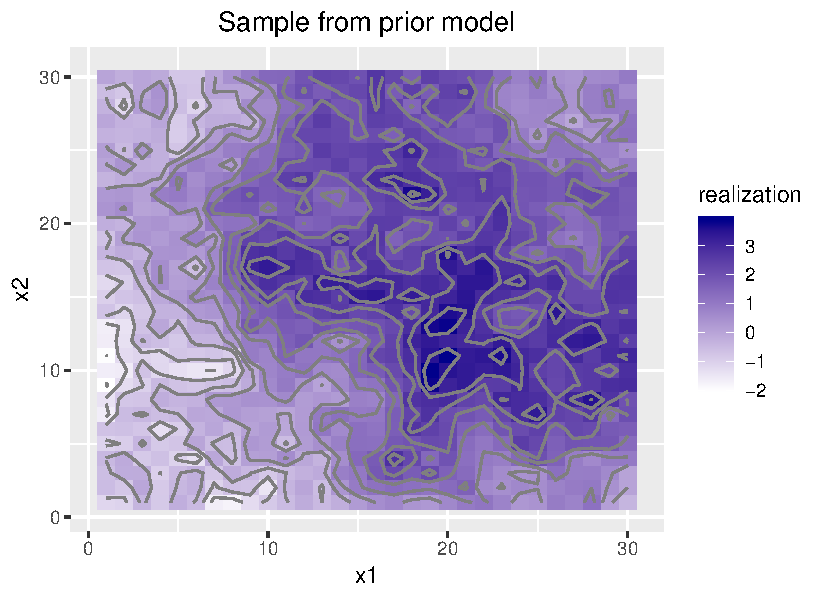
\includegraphics[scale=0.95]{figures/3a_realization.pdf}
    \caption{One realization of the discretized Gaussian RF given in \ref{sec:problem3}a.}
    \label{fig:3a_realization}
\end{figure}

%%%%%%%%%%%%%%%%%%%%%%%%%%%%%%%%%%%%%%%%%%%%%%%%%%%%%%%%%%%%%%%%%%%%%%
\paragraph{b)}
The variogram function for the Gaussian RF is
%
\begin{align*}
\gamma_r(\tau)
\coloneqq&\: \frac{1}{2} \Var \{ r(x) - r(x') \} \\
=&\: \sigma_r^2 - \Cov\{r(x), r(x')\} \\
=&\: \sigma_r^2 [1 - \exp\{-\tau/\xi_r\}] \, .
\end{align*}
%
This is shown in figure~\ref{fig:3b_variogram} together with the empirical variogram based on exact observations of the full realization in a). The empirical variogram is precise for small distances, but differs from the theoretical variogram for larger distances. This is not surprising, since there is less data for higher distances.

\begin{figure}
    \centering
    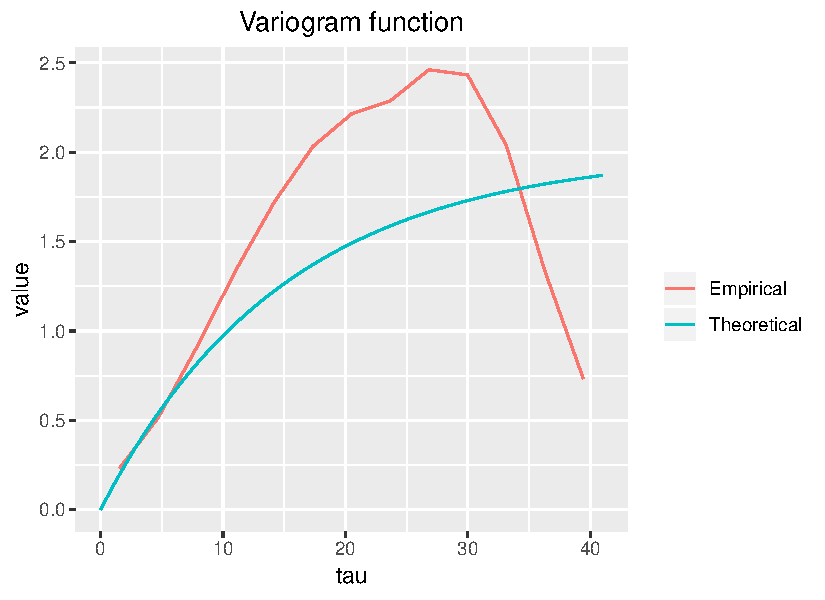
\includegraphics[scale=0.95]{figures/3b_variogram.pdf}
    \caption{The theoretical variogram and empirical variogram from one realization of the discretized Gaussian RF given in \ref{sec:problem3}a.}
    \label{fig:3b_variogram}
\end{figure}

%%%%%%%%%%%%%%%%%%%%%%%%%%%%%%%%%%%%%%%%%%%%%%%%%%%%%%%%%%%%%%%%%%%%%%
\paragraph{c)}
We generate 36 locations uniformly randomly on the grid $\mathrm{L}$ and compute the empirical variogram based on the realization values in these locations. See figure~\ref{fig:3c_variogram_obs}It is less smooth than the empirical variogram computed from the entire realization, but still quite close to the theoretical variogram for small distances.

\begin{figure}
    \centering
    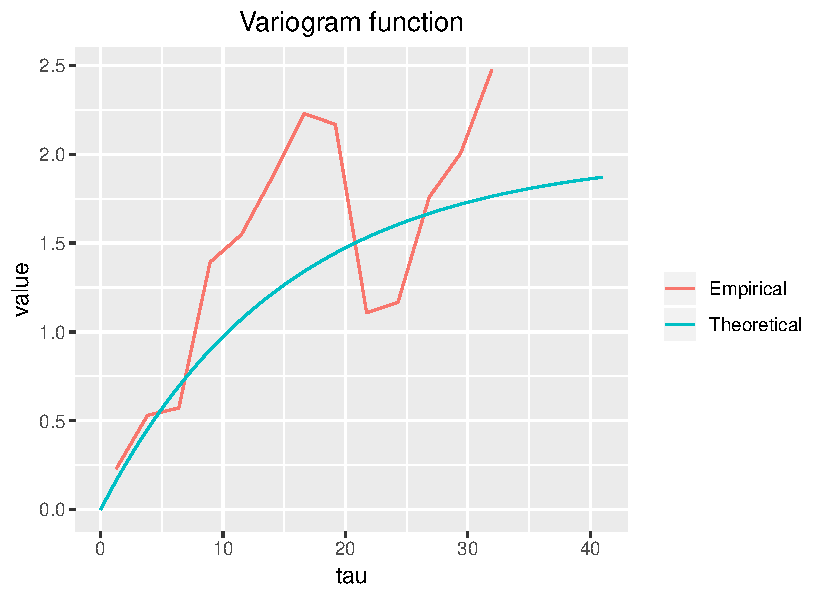
\includegraphics[scale=0.95]{figures/3c_variogram_obs.pdf}
    \caption{The theoretical variogram of the discretized Gaussian RF given in \ref{sec:problem3}a and the empirical variogram based on 36 exact randomly chosen observations of a realization.}
    \label{fig:3c_variogram_obs}
\end{figure}

Now we consider $\sigma_r^2$ and $\xi_r$ to be unknown and estimate their values by maximum likelihood estimation. We do this for the full realization and the 36 exact observations. This gives $\sigma_r^2 \approx 2.220$ and $\xi_r \approx 19.950$ using the full realization, and $\sigma_r^2 \approx 2.374$ and $\xi_r \approx 20.558$ using the observations. 

From these values we estimate the variogram function. They are displayed in figure~\ref{fig:3c_variogram_estimates}. The estimates are way more accurate and smooth than the empirical variograms. We can get a similarly smooth estimate by simulating several times and using the mean of the empirical variograms. This, however, takes a lot more time, and it is not possible if one doesn't know the true distribution and thus can't simulate repeatedly. For realizations of a higher resolution the empirical variogram would likely fare better.

\begin{figure}
    \centering
    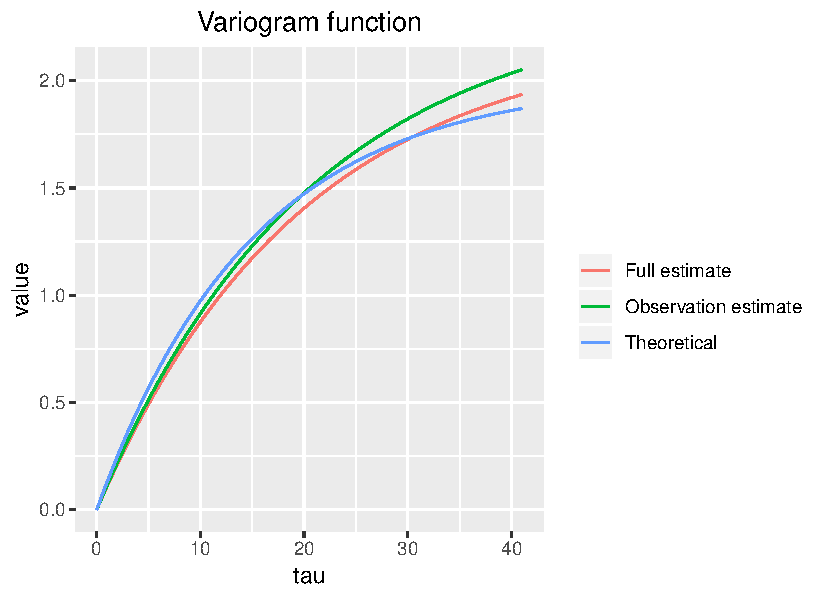
\includegraphics[scale=0.95]{figures/3c_variogram_estimates.pdf}
    \caption{The theoretical variogram of the discretized Gaussian RF given in \ref{sec:problem3}a and estimated variograms based on estimates of $\sigma_r^2$ and $\xi_r$ using the whole realization and using 36 observations.}
    \label{fig:3c_variogram_estimates}
\end{figure}

%%%%%%%%%%%%%%%%%%%%%%%%%%%%%%%%%%%%%%%%%%%%%%%%%%%%%%%%%%%%%%%%%%%%%%
\paragraph{d)}

\begin{figure}
    \centering
    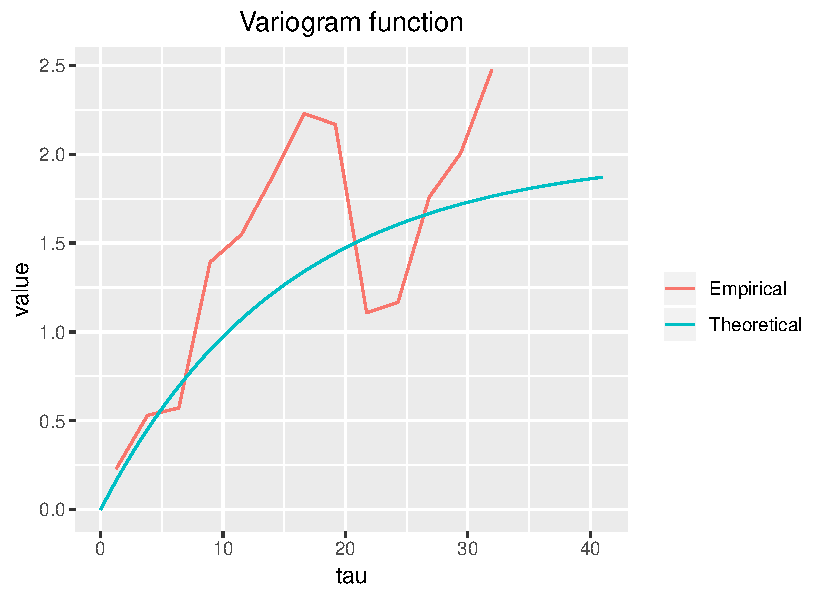
\includegraphics[scale=0.95]{figures/3c_variogram_obs.pdf}
    \caption{The theoretical variogram of the discretized Gaussian RF given in \ref{sec:problem3}a and the empirical variogram based on 36 exact randomly chosen observations of a realization.}
    \label{fig:3c_variogram_obs}
\end{figure}

Now we consider $\sigma_r^2$ and $\xi_r$ to be unknown and estimate their values by maximum likelihood estimation. We do this for the full realization and the 36 exact observations. This gives $\sigma_r^2 \approx 2.220$ and $\xi_r \approx 19.950$ using the full realization, and $\sigma_r^2 \approx 2.374$ and $\xi_r \approx 20.558$ using the observations. 

From these values we estimate the variogram function. They are displayed in figure~\ref{fig:3c_variogram_estimates}. The estimates are way more accurate and smooth than the empirical variograms. We can get a similarly smooth estimate by simulating several times and using the mean of the empirical variograms. This, however, takes a lot more time, and it is not possible if one doesn't know the true distribution and thus can't simulate repeatedly. For realizations of a higher resolution the empirical variogram would likely fare better.

\begin{figure}
    \centering
    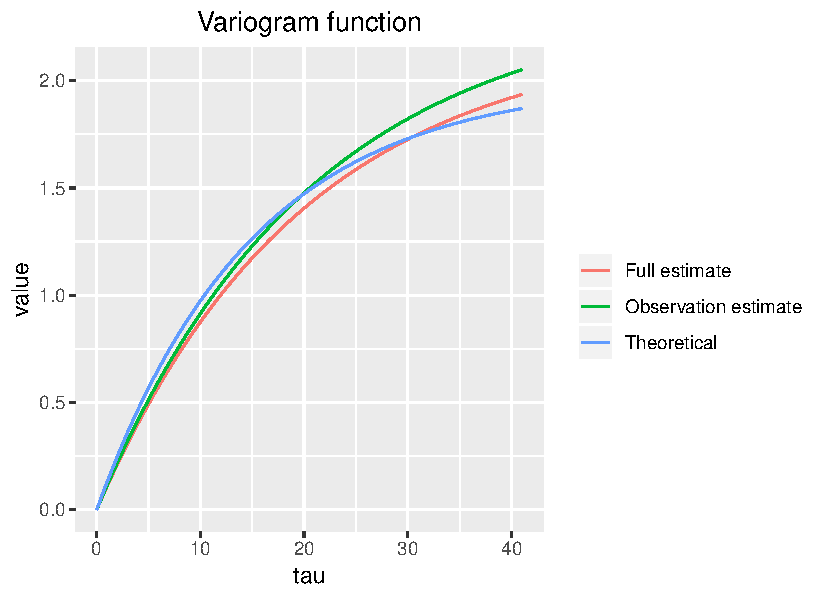
\includegraphics[scale=0.95]{figures/3c_variogram_estimates.pdf}
    \caption{The theoretical variogram of the discretized Gaussian RF given in \ref{sec:problem3}a and estimated variograms based on estimates of $\sigma_r^2$ and $\xi_r$ using the whole realization and using 36 observations.}
    \label{fig:3c_variogram_estimates}
\end{figure}

%%%%%%%%%%%%%%%%%%%%%%%%%%%%%%%%%%%%%%%%%%%%%%%%%%%%%%%%%%%%%%%%%%%%%%
\paragraph{e)}
text text text
